\chapter{Multi-layer Multiple Kernel Learning}
\label{chap_mlmkl}
In this chapter we  discuss the Multi-layer Multiple Kernel Learning (ML-MKL\nomenclature{ML-MKL}{Multi-layer Multiple Kernel Learning}) framework developed using an unsupervised MKL algorithm. The organization of this chapter is as follows;  section \ref{sec_mkl} gives  the discussion of  traditional MKL algorithm  in a supervised learning settings, in section \ref{sec_umkl} the unsupervised MKL formulation is introduced, in section \ref{sec_rw} the related works in ML-MKL domain is discussed, in section \ref{sec_mlmkl} the proposed ML-MKL algorithm is discussed along with the experimental results and section \ref{sec_conc} concludes this chapter.


\section{Multiple Kernel Learning}
\label{sec_mkl}
Multiple Kernel Learning(MKL\nomenclature{MKL}{Multiple Kernel Learning}) aims at learning a convex combination of a set of predefined base kernels for choosing an optimum kernel(\cite{mkl} et al.). The primary aim of MKL algorithm is to automate the process of choosing the optimum kernel  for the learning task.


Typically multiple kernel learning is formulated in a supervised learning settings. Suppose we are given $n$ datapoints $\mathcal{D} = \{(x_1, y_1), (x_2, y_2), \ldots, (x_n, y_n)\}$, where $x_i \in \mathbb{R}^d$ is the $i^{th}$ input data vector and $y_i$ is the label of the class to which $x_i$ belongs to. Then the MKL learning task is formulated as the following optimization problem.
\begin{equation}
\min_{k \in \mathcal{K}} \min_{f \in \mathcal{H}_k} \lambda \norm{f}^2_{\mathcal{H}_k} + \sum_{i=1}^n l(y_i, f(x_i))
\end{equation}
where $l(\cdot)$ denotes the loss function(commonly used loss function is the hinge loss, defined as $l(t) = \max(0, 1-t)$), $\mathcal{H}_k$ is the RKHS corresponding to the kernel $k$, $\mathcal{K}$ denotes the optimization domain of the candidate kernels, and $\lambda > 0$ is the regularization parameter.

The optimizaion domain $\mathcal{K}$ is the convex combination of a set of predefined base kernels, defined as follows
\[ \mathcal{K} = \Bigg\{ k( \cdot \textrm{ , } \cdot ) = \sum_{t=1}^m \mu_t k_t(\cdot \textrm{ , } \cdot) \textrm{ : } \sum_{t=1}^m \mu_t = 1, \mu_t \geq 0 \Bigg\} \]
where $k_t$ is the $t^{th}$ base kernel and $\mu_t$ is the weight associated to the $t^{th}$ base kernel. The decision function $f(x)$ can be computed as a linear combination of kernel evaluations on all training samples;
\[ f(x) = \sum_{i=1}^n \alpha_i k(x_i, x) \]
where $\alpha_i$'s are the coefficients. As per the definition of kernel $k$ in MKL, the decision function of the conventional MKL is expressed as
\begin{equation*}
\begin{aligned}
f(x) &= \sum_{i=1}^n \alpha_i \sum_{t=1}^m \mu_t k_t(x_i, x) \\
&= \sum_{i=1}^n \sum_{t=1}^m \alpha_i \mu_t k_t(x_i, x)
\end{aligned}
\end{equation*}
In this basic formulation, the optimization task has to identify both the optimal kernel $k$ from the domain $\mathcal{K}$ and the optimal decision function $f$ from the RKHS $\mathcal{H}_k$ simultaneously. In order to eliminate this problem \cite{corinna} et al. proposed a two stage kernel learning algorithm which separates the kernel learning task from the decision function learning.


\section{Unsupervised MKL}
\label{sec_umkl}
In the KPCA based feature extraction stages, we were using only one kernel for the task. With the intuition that by using multiple kernels at each layer we would get more similarity information, we computed a convex combination of multiple kernels following the work in \cite{zhuang} et al. Since we are using kernels for unsupervised feature extraction, traditional MKLs following supervised paradigm cannot be used here.

The goal of an unsupervised multiple kernel learning task is to find an optimal linear combination of the $m$ kernel functions as, i.e, $k^*(\cdot \textrm{ , } \cdot) \in \mathcal{K}$. %where $K$ is defined as follows:
%\[ K = \Bigg\{ k( \cdot \textrm{ , } \cdot ) = \sum_{t=1}^m \mu_t k_t(\cdot \textrm{ , } \cdot) \textrm{ : } \sum_{t=1}^m \mu_t = 1, \mu_t \geq 0 \Bigg\} \]  
%here $k_t$'s are the base kernels. 
In order to determine the optimality of a linear combination of kernels, we used the following quality criteria\cite{zhuang} et al.:

\begin{itemize}
\item A  good kernel should enable each training instances to be well reconstructed from the localized bases weighted by the kernel values. Formulating this requirment mathematically, for each $x_i$ we expect the optimal kernel should minimize the approximation error $\norm{x_i-\sum_j k_{ij}x_j}^2$, where $k_{ij} = k(x_i, x_j)$.
\item A good kernel should induce kernel values that are coincided with the local geometry of the training data. This is equivalent to finding the optimal kernel that minimizes the distortion over all trainig data, computed as $\sum_{i,j}k_{ij} \norm{x_i-x_j}^2 $.
\end{itemize}

In addition to this, the locality preserving principle can be exploited  by using a set of local bases for each $x_i \in X$ denoted as $B_i$. By fixing the size of the local bases to some constant $N_B$,  the optimization problem of unsupervised MKL can be formulated as follows.
\[ \min_{k \in \mathcal{K}} \frac{1}{2}\sum_{i=1}^n \norm{x_i - \sum_{x_j \in B_i} k_{ij}x_j}^2 + \gamma* \sum_{i=1}^n \sum_{x_j \in B_i} k_{ij} \norm{x_i-x_j}^2 \]

where $\gamma$ is a tuning parameter, which controls the tradeoff between the coding error and the locality distortion. Converting to matrix notations the above problem becomes
\begin{equation}
  \min_{\mu \in \Delta,D} \frac{1}{2} \norm{X(I-K \circ D)}_F^2 + \gamma* \textrm{ tr }K\circ D\circ M(11^T)
  \label{obj_mat} 
\end{equation}
%\begin{equation*}
 % \begin{aligned}
\[ \textrm{subject to } D \in \{0,1\}^{n \times n} \]
\[  \norm{d_i}_1 = N_B, i=1,2,\ldots,n \]
\[ \Delta = \Big\{\mu : \mu^T\textbf{1} = 1, \mu \geq 0 \Big\} \textrm{ and } \]
\[ [K]_{i,j} = \sum_{t=1}^m \mu_t k^t(x_i, x_j), 1\leq i,j \leq n \]
  %\end{aligned}
%\end{equation*}

The matrix $D \in \{0,1\}^{n \times n}$ contains information about local bases of each $x_i$ as a column vector. In particular, each column vector $d_i \in \{0, 1\}^n $ in $D$ has a 1 at those points $j$ where, $x_j \in B_i$ and zero elsewhere(or $B_i = \{ x_j : d_j \neq 0 \} $). The matrix M is defined as
\[ [M]_{ij} = x_i^Tx_i + x_j^Tx_j - 2x_i^Tx_j \]

In equation \ref{obj_mat} the notation `$\circ$' denotes elementwise multiplication of two matrices, $\norm{\cdot}_F^2$ denotes the Frobenius norm of a matrix and `tr' denotes the trace of a matrix.

In their implementation(\cite{zhuang}) Zhuang et.al solved the optimization problem in two stages in an alternating fashion, first by solving for $\mu$ with a fixed $D$ (using convex optimization) and then solving for $D$ by fixing $\mu$ (using a greedy mixed integer programming formulation). Since we are using a many layer architecture, the alternating optimization strategy is too costly; so we chose to do the optimization across $\mu$ only by choosing $D$ beforehand. Specifically, the matrix $D$ is computed beforehand by taking $k$ nearest neighbours of $x_i$ from the training set and putting a one in those positions for $d_i$. Rest of the positions are filled with zeros. The resulting optimization problem will be  
\begin{equation}
  \begin{aligned}
  \min_{\mu \in \Delta} \frac{1}{2} \norm{X(I-K \circ D)}_F^2 + \gamma* \textrm{ tr }K\circ D\circ M(11^T)
  \end{aligned}
\end{equation}
\[ \textrm{subject to } D \in \{0,1\}^{n \times n}, \norm{d_i}_1 = N_B, i=1,2,\ldots,n \]
\[ \Delta = \Big\{\mu : \mu^T\textbf{1} = 1, \mu \geq 0 \Big\} \]

The objective function can be formulated as a convex quadratic programming problem w.r.t to kernel weights $\mu$ as shown below(derivation of the objective function $J(\mu)$ is shown in Appendix \ref{derivation1}).
\begin{equation}
J(\mu) = \mu^T \Bigg( \sum_{t=1}^m \sum_{i=1}^n k_{t,i}k_{t,i}^T \circ d_i d_i^T \circ P \Bigg)^T \mu + z^T \mu 
\end{equation}
where $[z]_t = \sum_{i=1}^n (2 \gamma v_i \circ d_i - 2 p_i \circ d_i)^T \mathit{k}_{t,i} $, $P = X^TX$, and $\mathit{k}_{t,i} = \Big[ k^t(x_i, x_1), \ldots, k^t(x_i, x_n) \Big]^T $ is the $i^{th}$ column of the $t^{th}$ kernel matrix. $p$ and $v$ are columns of $P$ and $M$ corresponding to $x_i$ respectively.

\section{Related Works}
\label{sec_rw}

\cite{2l_mkl} et al. explored the idea of ML-MKL, in which at each layer they took a non-linear combination of kernels in the previous layer, forming a layered structure. They called such a model as deep multiple kernel learning framework. The architecture of their model is shown in figure \ref{fig_2l_mkl}. The kernel function obtained at layer $l$ is having the following domain.
\[ \mathcal{K}^{(l)} = \bigg\{ k^{(l)}(\cdot, \cdot) = g^{(l)}\Big( \big[k_1^{(l-1)},\ldots, k_m^{(l)}(\cdot, \cdot) \big] \Big)  \bigg\} \]

\begin{figure*}
  \centering
  \captionsetup{justification=centering,margin=0.1cm}
  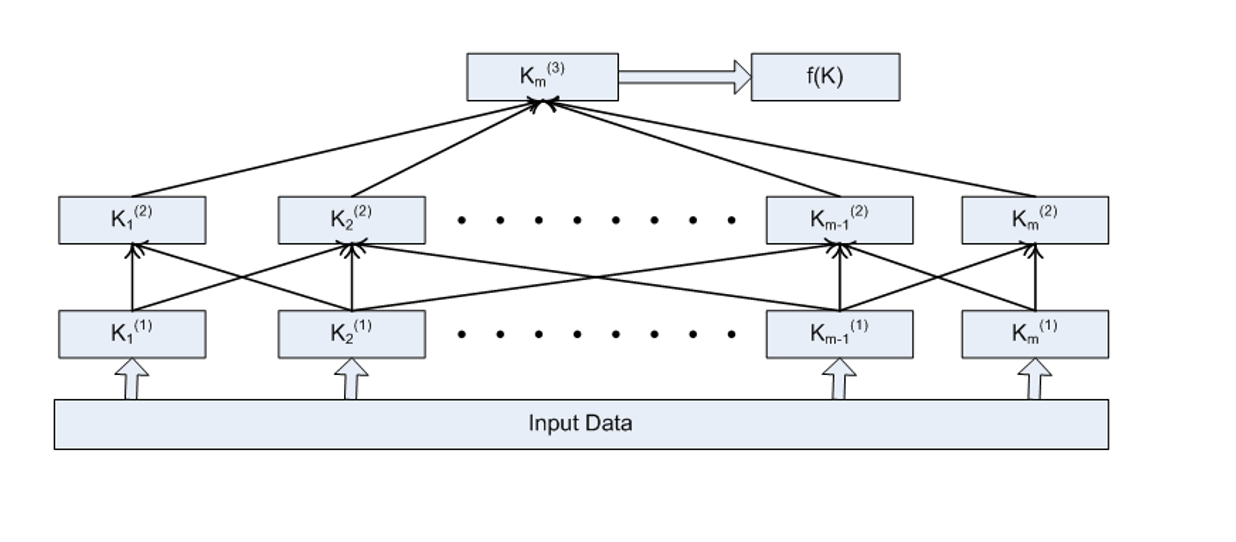
\includegraphics[width=1.1\textwidth,height=8.5cm]{figures/2lmkl}
  \caption{Architecture of ML-MKL model proposed by \cite{2l_mkl} et al.}
  \label{fig_2l_mkl}
\end{figure*}

where $g^{(l)}$ is a function to combine multiple $(l-1)$ level kernels, which must ensure the resulting combination is a valid kernel. Though this combination can be applied for any number of layers, optimization problem is difficult to solve beyond two layers. Hence \cite{2l_mkl} et al. considered only 2-layer MKL in their empirical study. 

In the 2-layer MKL, \cite{2l_mkl} et al. defined the kernel domain by using an RBF kernel for the combination function. 
\[ \mathcal{K}^{(2)} = \bigg\{ k^{(2)}(x_i, x_j;\bm{\mu}) = exp\Big( \sum_{t=1}^m \mu_t k_t^{(1)}(x_i, x_j) \Big)  \bigg\}  \colon \bm{\mu} \in \mathbb{R}_+^m \]
$\mu_t$ is the weight of the $t^{(th)}$ antecedent layer kernel $k_t^{(1)}$(superscript (1) is used here because the antecedent layer is layer 1 in a 2-layer architecture). In order to prevent the kernel weight being too large, the kernel weights are also introduced into the optimization objective as a regularization term. Then the optimization objective becomes
\begin{equation}
\min_{k \in \mathcal{K}} \min_{f \in \mathcal{H}_k} \norm{f}^2_{\mathcal{H}_k} + \mathcal{C} \sum_{i=1}^n l(y_i, f(x_i)) + \sum_{t=1}^m \mu_t
\end{equation}
solving the Lagrangian, we will get the dual objective function as
\[ \min_{\bm{\mu}} \max_{\bm{\alpha}} \sum_{i=1}^n \alpha_i - \frac{1}{2}\sum_{i,j=1}^n \alpha_i \alpha_j y_i y_j k^{(2)}(x_i, x_j;\bm{\mu}) + \sum_{t=1}^m \mu_t \]
\[ \textrm{s.t } 0\leq \alpha_i\leq \mathcal{C}, \sum_{i=1}^n \alpha_i y_i = 0, \mu_t \geq 0, t=1, \ldots, m \]
where $\alpha = [\alpha_1, \alpha_2, \ldots, \alpha_n]^T$ is a vector of dual variables and $\mu = [\mu_1, \mu_2, \ldots, \mu_m]^T$. The final decision function of the 2-layer MKL is given as
\[f(x;\bm{\alpha}, \bm{\mu}) = \sum_{i=1}^n \alpha_i y_i k^{(2)}(x_i, x;\bm{\mu}) + b \]
where $b$ is the bias term. Rewriting the optimization objective in terms of $\alpha$ and $\mu$, we have
\[ \mathcal{J}(\alpha, \mu) = \frac{1}{2} \sum_{i,j=1}^n \alpha_i \alpha_j y_i y_j k^{(2)}(x_i, x_j;\bm{\mu}) - \sum_{i=1}^n \alpha_i - \sum_{t=1}^m \mu_t \]
The optimization problem is solved in two stages
\begin{itemize}
\item by fixing $\mu$ and solve for $\alpha$.
\item by fixing $\alpha$ and solve for $\mu$.
\end{itemize}
Since $k^{(2)}$ is positive definite $\mathcal{J}(\alpha, \mu)$ is convex over $\alpha$, thus an SVM solver can be used to solve the optimization over $\alpha$. The optimization over $\mu$ is solved using gradient ascent. In order to address the challenge of choosing the optimal set of base kernels, they proposed to choose base kernels iteratively inside $k^{(2)}$.

\cite{deep_mkl} et al. used backpropagation algorithm for designing the ML-MKL framework. The architecture of the model studied by them is shown in figure \ref{fig_deep_mkl}. They defined the kernel domain at level $l$ as

\begin{figure*}
  \centering
  \captionsetup{justification=centering,margin=0.1cm}
  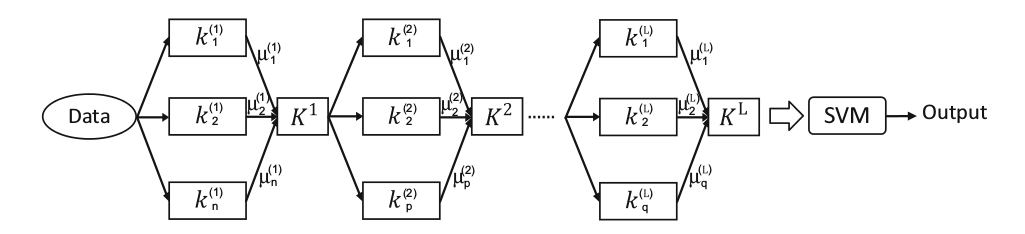
\includegraphics[width=1\textwidth,height=6cm]{figures/back_prop_mlmkl}
  \caption{Architecture of ML-MKL model proposed by \cite{deep_mkl} et al. The kernels in each layer are linearly combined and the resulting Gram matrix is passed to the next layer as input.}
  \label{fig_deep_mkl}
\end{figure*}

\[ \mathcal{K}^{(l)} = \big\{ K^{(l)}(K^{(l-1)}; \mu^{(l)}) = \sum_{t=1}^m \mu_t^{(l)} k_t^{(l)}(K^{(l-1)})  \big\} \]
\[ \textrm{s.t } \mu_t^{(l)} \geq 0, l = 1, \ldots, L \]
where $k_t^{(l)}$ is the $k^{th}$ base kernel at layer $l$ and $\mu_t^{(l)}$ denotes the weight of the $k^{th}$ base kernel at layer $l$. $L$ is the total number of layers. The feature extracted in the antecedent layer are combined linearly and passed to the next layer as input. The kernel weights are obtained by minimizing the mean squre error(denotes as $\mathcal{E}$) of the predicted outputs.
\[ \mathcal{E} = \frac{1}{2n} \sum_{i=1}^n \norm{f(x_i) - y_i}^2 \]
where $f(x_i)$ is the value of the decision function for the input $x_i$, which is computed as
\[ f(x) = \sum_{i=1}^n \alpha_i y_i K^{(l)}(K^{(l-1)}; \mu^{(l)}) + b \]
where $b$ is the bias term. The weights $\mu^{(l)}$ in each layer are obtained using gradient descent algoritm.
\[ \mu^{(l)} := \mu^{(l)} + \eta \nabla \mathcal{E}  \textrm{ } l = 1, \ldots, L \]
\[ \nabla \mathcal{E} = \Bigg\{ \frac{\partial \mathcal{E}}{\partial \mu_1^{(1)}}, \cdots, \frac{\partial \mathcal{E}}{\partial \mu_m^{(1)}}; \cdots; \frac{\partial \mathcal{E}}{\partial \mu_1^{(L)}}, \cdots, \frac{\partial \mathcal{E}}{\partial \mu_m^{(L)}}  \Bigg\}  \]
Here $\eta$ is the learning rate parameter. The error obtained in the final layer are propagated back to all layers using backpropagation algorithm to update the kernel weight parameters $\mu^{(l)}$ in each layer.

\section{Multi-layer Multiple Kernel Learning}
\label{sec_mlmkl}
The architectue of the proposed ML-MKL framework is shown in figure \ref{fig_mlmkl}. It consists of many layers and in each layer the kernel PCA based feature extraction is performed using the combination of a set of predefined kernels. The dimensionality of the features thus obtained are reduced by using supervised feature selection techniques. The final output can be given to any classifier. Algorithm \ref{algo1} summarizes the proposed ML-MKL algorithm.

\begin{algorithm}
\caption{ML-MKL Algorithm}
\textbf{Input}: data X, true labels y, no. of layers L, base kernels for each layer $K_{base}^{(l)} = \{k_1^{(l)}, k_2^{(l)}, k_m^{(l)}\}$, $N_B$, $\gamma$\;
\textbf{Output}: kernel weights $\mu^l$ for each layer, predicted labels\;
1.Initialize $[M]_{ij} = x_i^Tx_i + x_j^Tx_j - 2x_i^Tx_j$, $\bm{D} = d_1, d_2, \ldots, d_n$ as row vectors, where $d_i = \{1 \textrm{ if } x_j \in B_i \textrm{ else } 0 \forall x_j \in X \}$, $\mu = \frac{1}{m}$, $\bm{P} = X^TX$\;
2.\For{each layer l}{
    a. $\bm{W} = \sum_{t=1}^m \sum_{i=1}^n k_{t,i}^{(l)}k_{t,i}^{(l)^{T}} \circ d_i d_i^T \circ P$\\
    b. $\bm{[z]}_t^l = \sum_{i=1}^n (2 \gamma v_i \circ d_i - 2 p_i \circ d_i)^T \mathit{k}_{t,i}^{(l)}$\\
    c. $\bm{\mu}^{*^{l}} = \mu^{l^{T}}W\mu^l + z^{l^{T}}\mu^l$\\
    d. $\bm{K}_{new} = \sum_{t=1}^m \mu_t^l * K_t^{(l)}$\\
    e. extract principal components with $\bm{K}_{new}$\\
    f. select most informative features for layer $l$($X_{new}$)\\
    g. $\bm{P} = X_{new} ^T X_{new}$
}
3.Give the final set of features to any classifier\;
\label{algo1}
\end{algorithm}

\begin{figure*}
  \centering
  \captionsetup{justification=centering,margin=0.1cm}
  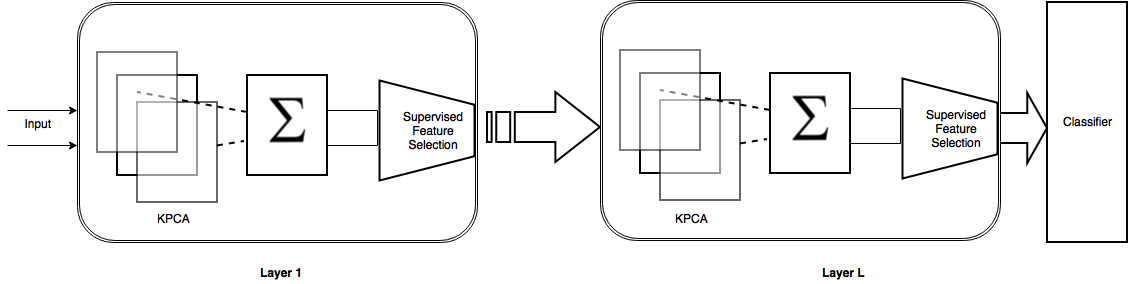
\includegraphics[width=1.0\textwidth,height=5.5cm]{figures/mlmkm}
  \caption{An ML-MKL with L layers of transformations. Each layer consists of many kernels for feature  extraction using kernel PCA and a supervised feature selection module.}
  \label{fig_mlmkl}
\end{figure*}

The experimental setup used here was the same as described in \autoref{chap_mkm}. Table \ref{tab_mlmkl} lists the results obtained with the proposed ML-MKL framework. The classifier used was  SVM with arc-cosine kernel. For \textit{mnist-back-rand} dataset, the best result was obtained with a model consists of 4 layers and in each layer 7 kernels were used. In particular, each layer consisted of a mixture of one arc-cosine kernel and 6 gaussian kernels. For \textit{mnist-back-image} dataset, the best ML-MKL model obtained had 2 layers and 5 kernels in each layer. In each layer a mixture of one arc-cosine kernel and 4 polynomial kernels were used. In the case of \textit{mnist-rot-back-image} dataset the best result was fetched by a model having only one layer with 4 arc-cosine kernels in it. For \textit{rectangles-image} dataset the best result was shown by a one layer ML-MKL model with one arc-cosine kernel and 6 Gaussian kernels.


\renewcommand{\arraystretch}{2.1}
\begin{table*}
\centering
\begin{tabular}{|c|c|c|c|c|c|c|c|}
  \hline
  \multirow{2}{*}{\textbf{Dataset}} & \multicolumn{7}{ |c| }{\textbf{Loss in Percentage}} \\
  \cline{2-8}
  &$\textrm{SVM}_{\textrm{RBF}}$ & $\textrm{SVM}_{\textrm{Poly}}$ & NNet & DBN-3 & SAA-3 & DBN-1 & \textbf{ML-MKL}\\
  \hline  
  \textit{back-rand} & 14.58 & 16.62 & 20.04 & \textbf{6.73} & 11.28 & 9.80 & 8.43$\pm 0.088$\\
  \hline
  \textit{back-image} & 22.61 & 24.01 & 27.41 & 16.31 & 23.00 & \textbf{16.15} & 20.92$\pm 0.092$\\
  \hline
  \textit{rot-back-image} & 55.18 & 56.41 & 62.16 & \textbf{47.39} & 51.93 & 52.21 & 51.21$\pm 0.811$\\
  \hline
  \textit{rect-image} & 24.04 & 24.05 & 33.20 & 23.69 & 24.05 & \textbf{22.50} & 22.88$\pm 0.124$\\
  \hline
\end{tabular}
\caption{Experimental Results of ML-MKL.}
\label{tab_mlmkl}
\end{table*}
\renewcommand{\arraystretch}{1}

Figures \ref{fig_mbr_layers} and \ref{fig_mbi_layers} illustrates the variation in classifier performance on \textit{mnist-back-rand} and \textit{mnist-back-image} datasets respectively when layers were added iteratively to the ML-MKL model. The value shown for each layer was the best error rate obtained after tuning the kernel parameters. The parameters were chosen greedily for each layer (with the expectation that subsequent layers would learn more valuable features from the current one) and no fine-tuning was performed with respect to the entire architecture.

\begin{figure}
  \centering
  \captionsetup{justification=centering,margin=0.1cm}
  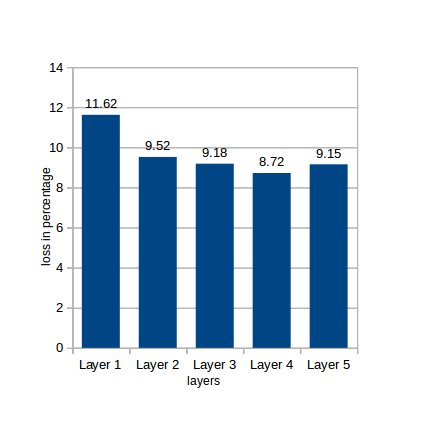
\includegraphics[scale=0.8]{figures/mlmkl_rand}
  \caption{Change in classifier performance on \textit{mnist-back-rand} dataset when adding layers iteratively.}
  \label{fig_mbr_layers}
\end{figure}

\begin{figure}
  \centering
  \captionsetup{justification=centering,margin=0.1cm}
  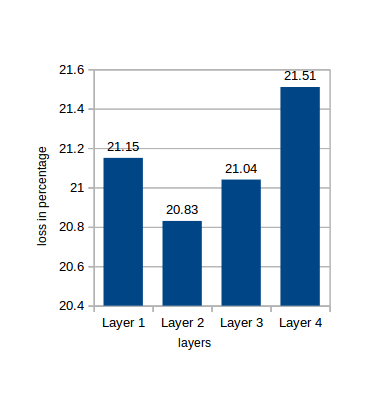
\includegraphics[scale=0.8]{figures/mlmkl_image}
  \caption{Change in classifier performance on \textit{mnist-back-image} dataset when adding layers iteratively.}
  \label{fig_mbi_layers}
\end{figure}

Figure \ref{tsne_rand_mlmkl} shows the tSNE embedding of the features learned by ML-MKL algorithm. The visualization indicates that classes are well separated.

\begin{sidewaysfigure}
  \centering
  \captionsetup{justification=centering,margin=0.1cm}
  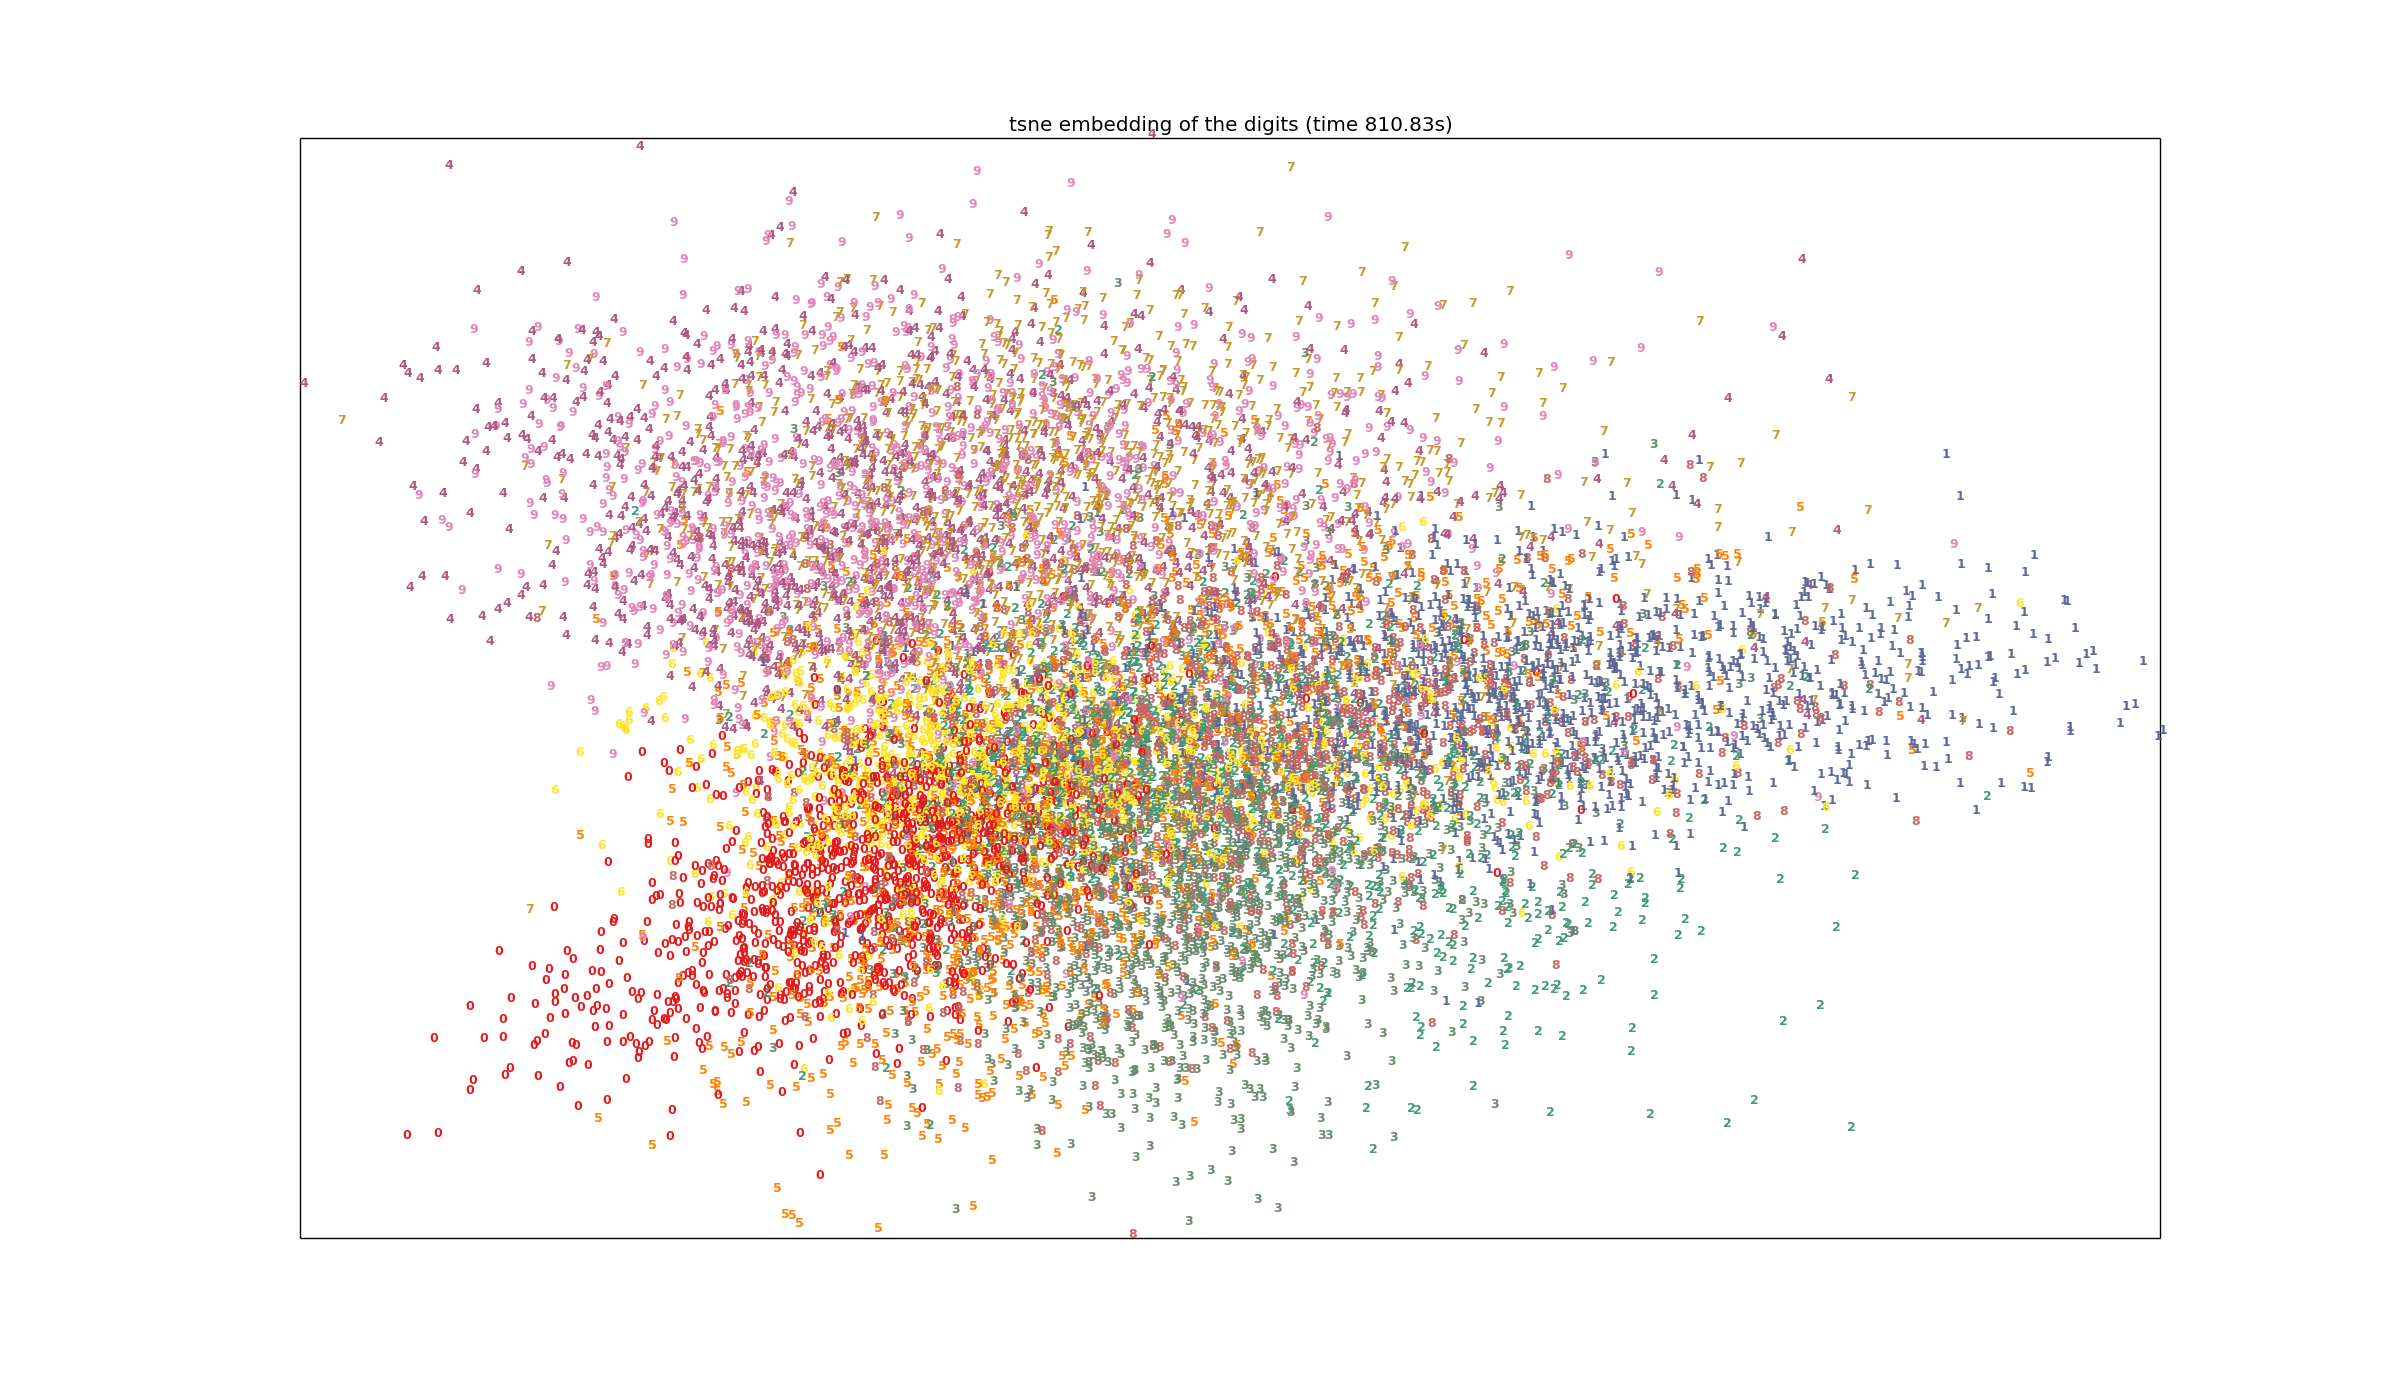
\includegraphics[scale=0.45]{figures/tsne_rand_mlmklbest}
  \caption{tSNE embedding of features obtained by ML-MKL algorithm for the \textit{mnist-back-rand} dataset.}
  \label{tsne_rand_mlmkl}
\end{sidewaysfigure}

Tables \ref{back_rand_kw} and \ref{back_image_kw} shows the kernel weights of each kernel in the mixture at every layer for \textit{mnist-back-rand} and \textit{mnist-back-image} datasets respectively. In both cases $k_1$ is an acr-cosine kernel, and the remaining are Gaussian kernels for \textit{mnist-back-rand} dataset and polynomial kernel for textit{mnist-back-image} dataset. The results in the table indicates that,  the contribution of individual kernels was highly varying in each layer (no single kernel had complete dominance over all layers in the feature learning process). 


\renewcommand{\arraystretch}{2.3}
\begin{table*}
\centering
\begin{tabular}{|c|c|c|c|c|c|c|c|}
  \hline
  \multirow{2}{*}{\textbf{Layers}} & \multicolumn{7}{ |c| }{\textbf{Kernel Weights}} \\
  \cline{2-8}
  & $k_1$ & $k_2$ & $k_3$ & $k_4$ & $k_5$ & $k_6$ & $k_7$ \\
  \hline  
  \textit{Layer 1} & 0.2007 & 0.1331 & 0.1331 & 0.1332 & 0.1332 & 0.1333 & 0.1333\\
  \hline
  \textit{Layer 2} & 0.2711 & 0.1160 & 0.1181 & 0.1203 & 0.1225 & 0.1248 & 0.1271\\
  \hline
  \textit{Layer 3} & 0.1764 & 0.0999 & 0.1125 & 0.1266 & 0.1426 & 0.1607 & 0.1811\\
  \hline
  \textit{Layer 4} & 0.0598 & 0.0524 & 0.0747 & 0.1071 & 0.1547 & 0.2245 & 0.3269\\
  \hline
  \textit{Layer 5} & 0.0514 & 0.0493 & 0.0726 & 0.1069 & 0.1569 & 0.2295 & 0.3334\\
  \hline    
\end{tabular}
\caption{Kernel weights in each layer for the \textit{mnist-back-rand} dataset}
\label{back_rand_kw}
\end{table*}
\renewcommand{\arraystretch}{1}

\renewcommand{\arraystretch}{2.3}
\begin{table}
\centering
\begin{tabular}{|c|c|c|c|c|c|}
  \hline
  \multirow{2}{*}{\textbf{Layers}} & \multicolumn{5}{ |c| }{\textbf{Kernel Weights}} \\
  \cline{2-6}
  & $k_1$ & $k_2$ & $k_3$ & $k_4$ & $k_5$\\
  \hline  
  \textit{Layer 1} & 0.2445 & 0.1887 & 0.1888 & 0.1889 & 0.1891\\
  \hline
  \textit{Layer 2} & 0.3421 & 0.1603 & 0.1630 & 0.1659 & 0.1688\\
  \hline
  \textit{Layer 3} & 0.2035 & 0.1615 & 0.1843 & 0.2104 & 0.2403\\
  \hline
  \textit{Layer 4} & 0.0843 & 0.1409 & 0.1877 & 0.2508 & 0.3362\\
  \hline
\end{tabular}
\caption{Kernel weights in each layer for the \textit{mnist-back-image} dataset}
\label{back_image_kw}
\end{table}
\renewcommand{\arraystretch}{1}

In order to evaluate the contribution of each kernel, exploratory analysis was carried out to monitor the performance of individual kernels in each layer. The individual kernels performance were compared with the combined kernel's performance. Tables \ref{back_rand_exp} and \ref{back_image_exp} summarizes the results of this exploratory analysis on \textit{mnist-back-rand} and \textit{mnist-back-image} datasets respectively (here $K_{conv}$ is the result of combined kernel). The results clearly indicates that the combination was not always improving the performance in all layers. However, the best result in both datasets were obtained by a combined kernel.

\renewcommand{\arraystretch}{2.1}
\begin{table*}
\centering
\begin{tabular}{|c|c|c|c|c|c|c|c|c|}
  \hline
  \multirow{2}{*}{\textbf{Layers}} & \multicolumn{8}{ |c| }{\textbf{Loss in Percentage}} \\
  \cline{2-9}
  & $k_1$ & $k_2$ & $k_3$ & $k_4$ & $k_5$ & $k_6$ & $k_7$ & $K_{conv}$\\
  \hline  
  \textit{Layer 1} & 11.46 & 9.92 & 10.06 & 10.04 & 10.1 & 9.87 & 10.06 & 11.62\\
  \hline
  \textit{Layer 2} & 10.36 & 9.87 & 9.90 & 9.89 & 9.92 & 9.82 & 9.81 & 9.52\\
  \hline
  \textit{Layer 3} & 9.46 & 11.07 & 10.33 & 9.85 & 9.70 & 9.56 & 9.01 & 9.18\\
  \hline
  \textit{Layer 4} & 9.26 & 9.06 & 8.95 & 8.96 & 8.93 & 8.72 & 9.00 & \textbf{8.72}\\
  \hline
  \textit{Layer 5} & 9.18 & 9.07 & 9.02 & 9.20 & 9.22 & 9.36 & 9.47 & 9.15\\
  \hline    
\end{tabular}
\caption{Individual kernels performance evaluation for \textit{mnist-back-rand} dataset}
\label{back_rand_exp}
\end{table*}
\renewcommand{\arraystretch}{1}

\renewcommand{\arraystretch}{2.1}
\begin{table}
\centering
\begin{tabular}{|c|c|c|c|c|c|c|}
  \hline
  \multirow{2}{*}{\textbf{Layers}} & \multicolumn{6}{ |c| }{\textbf{Loss in Percentage}} \\
  \cline{2-7}
  & $k_1$ & $k_2$ & $k_3$ & $k_4$ & $k_5$ & $K_{conv}$\\
  \hline  
  \textit{Layer 1} & 20.91 & 21.82 & 21.82 & 21.83 & 21.77 & 21.15\\
  \hline
  \textit{Layer 2} & 21.27 & 21.00 & 21.09 & 21.04 & 21.04 & \textbf{20.83}\\
  \hline
  \textit{Layer 3} & 20.95 & 21.18 & 21.02 & 20.99 & 21.05 & 21.03\\
  \hline
  \textit{Layer 4} & 21.06 & 21.36 & 21.42 & 21.64 & 21.66 & 21.51\\
  \hline
\end{tabular}
\caption{Individual kernels performance evaluation for \textit{mnist-back-image} dataset}
\label{back_image_exp}
\end{table}
\renewcommand{\arraystretch}{1}



\section{Conclusion}
\label{sec_conc}
In this chapter we explored the concept of multiple kernel learning in MKMs. A linear combination of multiple kernels formulated purely from unlabelled data is used in each layer of MKMs. The learning process of the proposed ML-MKL algorithm employs a greedy layerwise training for each layer. Empirical results indicates that using (unsupervised) MKL  in MKMs improves the classifier performance. In our experimental analysis the classification accuracy of ML-MKL models was better than learning machines with shallow architectures and was comparable with existing deep architectures.

Exploratory analysis performed on the features learned by the ML-MKL model reveals much more interesting facts about the model. The contribution of kernels in each layer is measured in terms of individual kernel performance and the weights assigned to that kernel. However this information is insufficient to determine the optimal structural complexity required for modelling a problem.
